\begin{figure}[h]
    \centering
    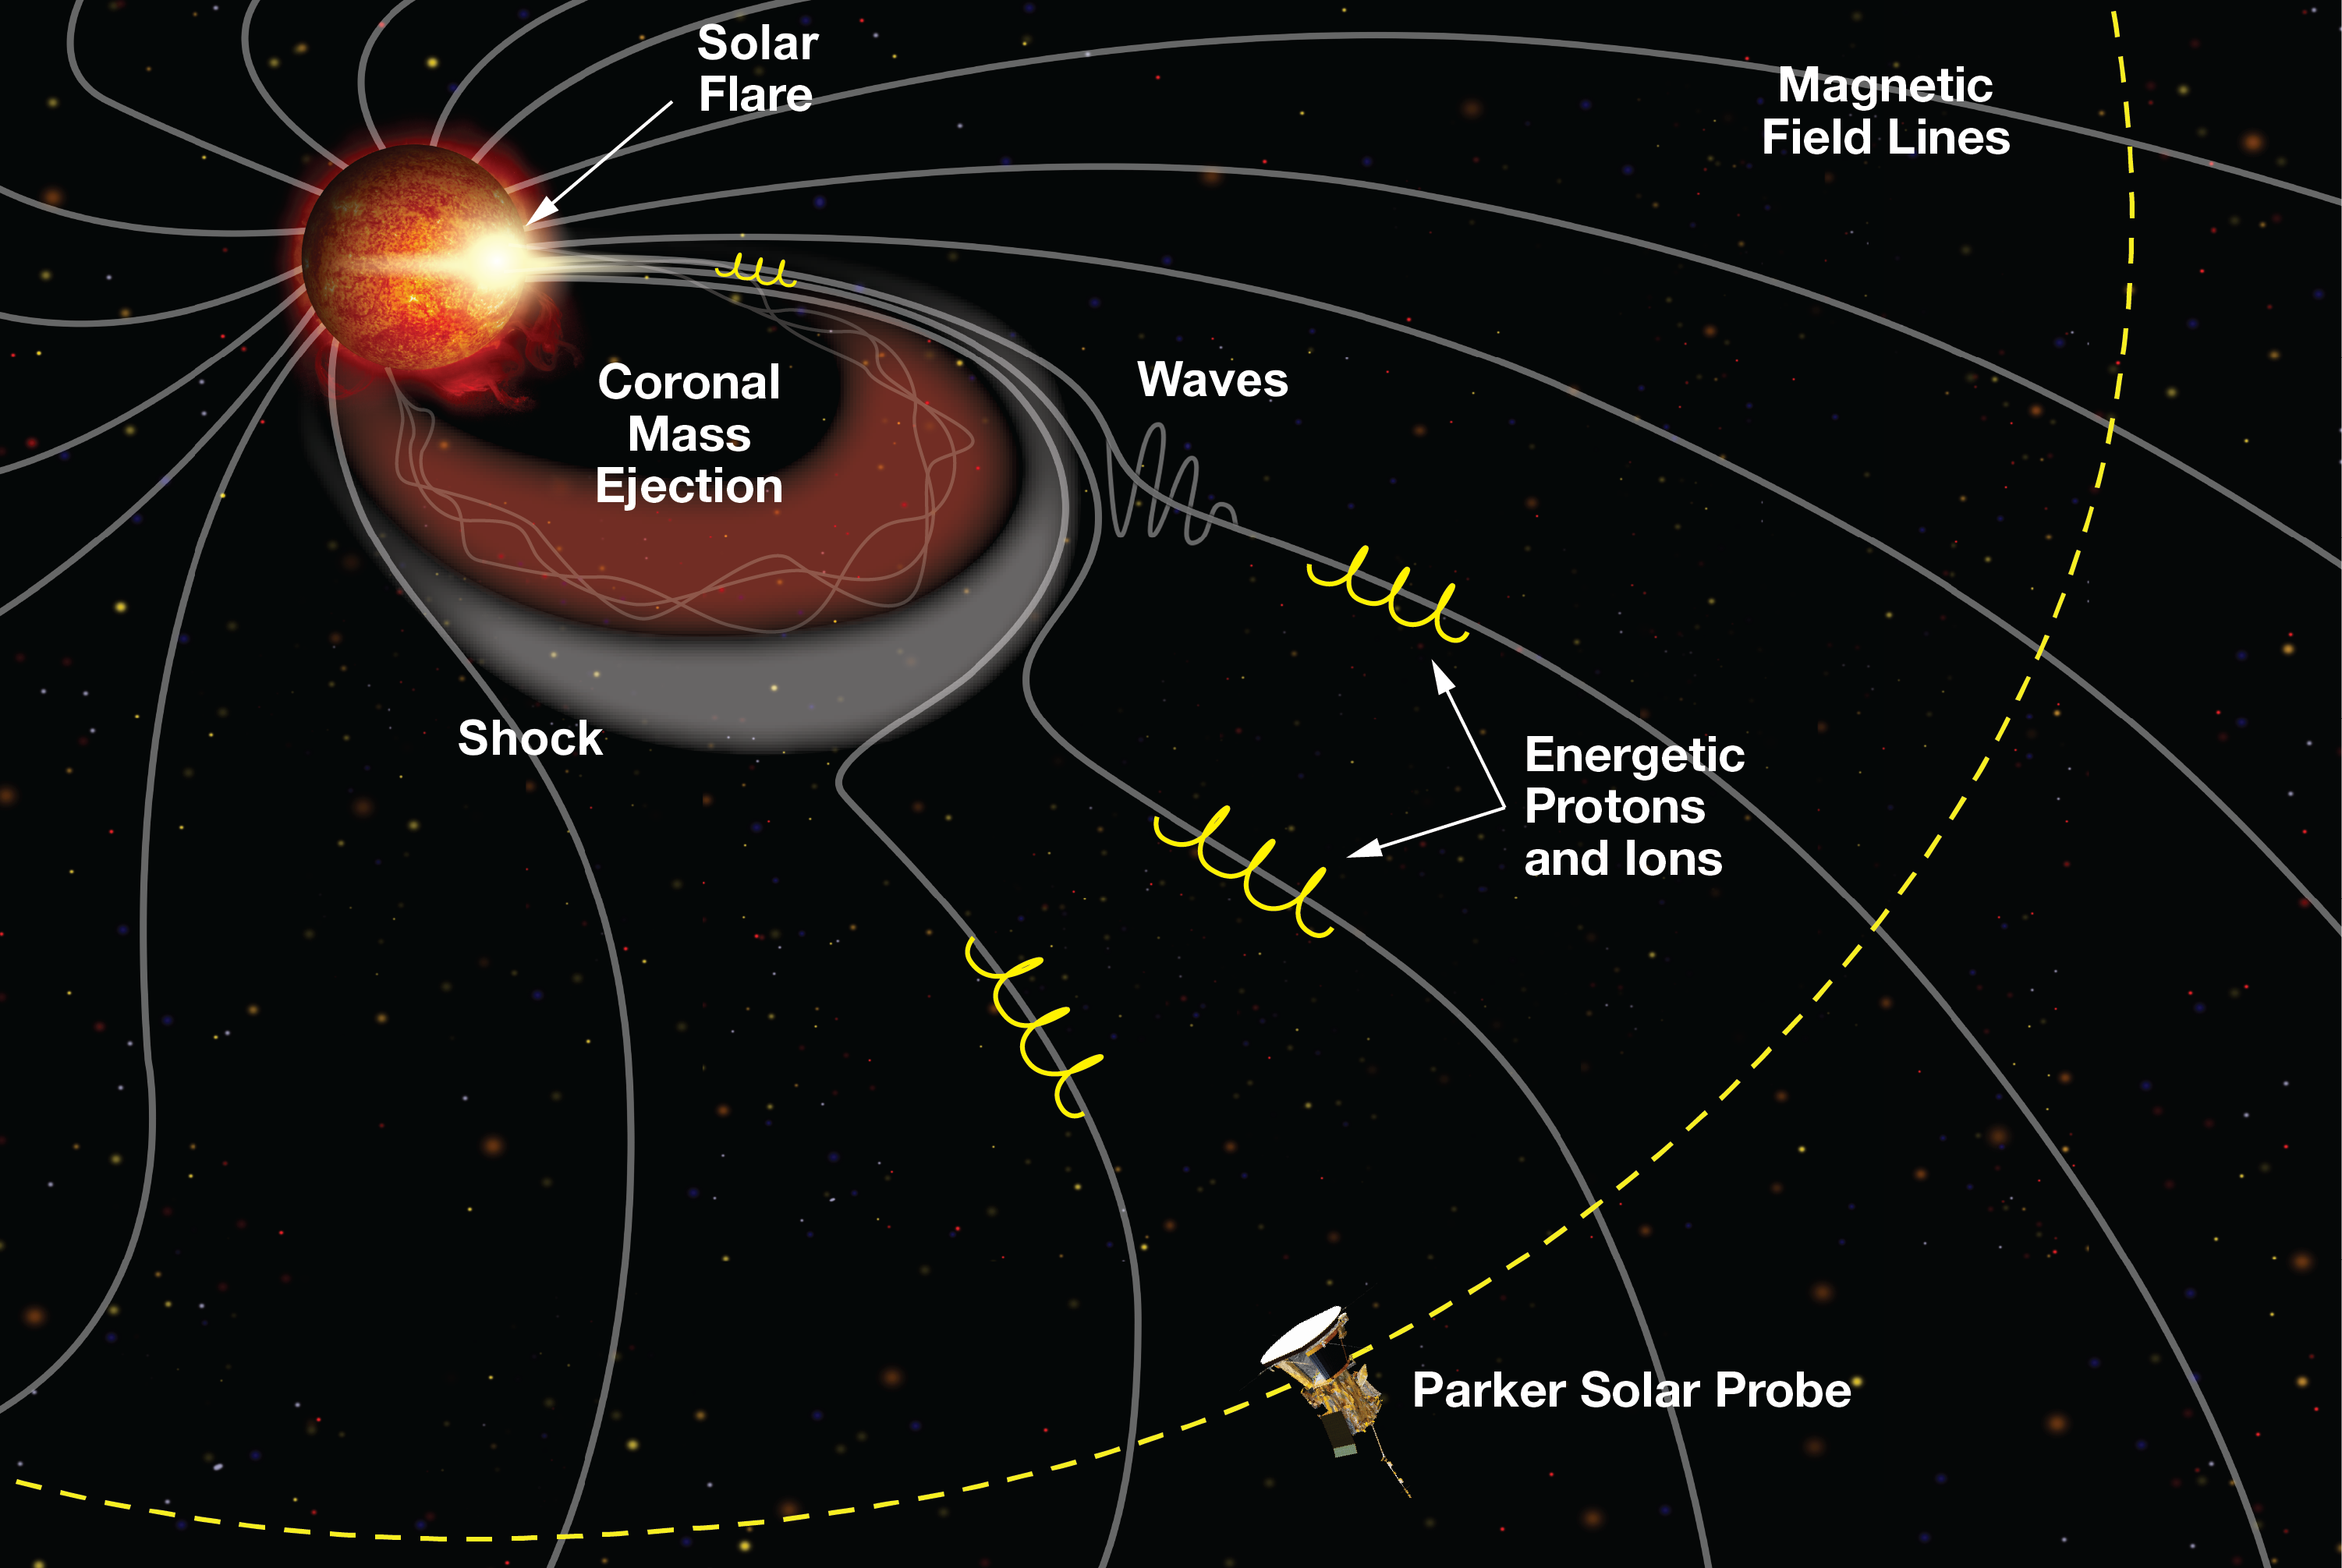
\includegraphics[width=0.7\textwidth]{parker_spirals.png}
    \caption{The spiral geometry of the solar wind and the
    interplanetary magnetic field lines (source: \cite{NASA}).}
    \label{fig:spirals}
\end{figure}

The solar wind originated from the solar corona is a magnetized
and nearly collisionless plasma consisting primarily of electrons, protons, and
alpha particles. Typically, it can be described as a magnetohydrodynamic fluid
with a very high magnetic Reynold's number. Consequently, the magnetic field at
the solar surface is frozen into the solar wind plasma and carried along with
it. This results in a spiraled geometry of the interplanetary magnetic field
lines called the Parker spirals (see \cref{fig:spirals}). \cite{Parker1958}
found from this geometry that the magnetic field followed an inverse square law
$B_r\sim r^{-2}$ and the particle density $n\sim r^{-2}V^{-1}$ also decreased
with increasing speed $V$ and radial distance $r$.

\begin{figure}
    \centering
    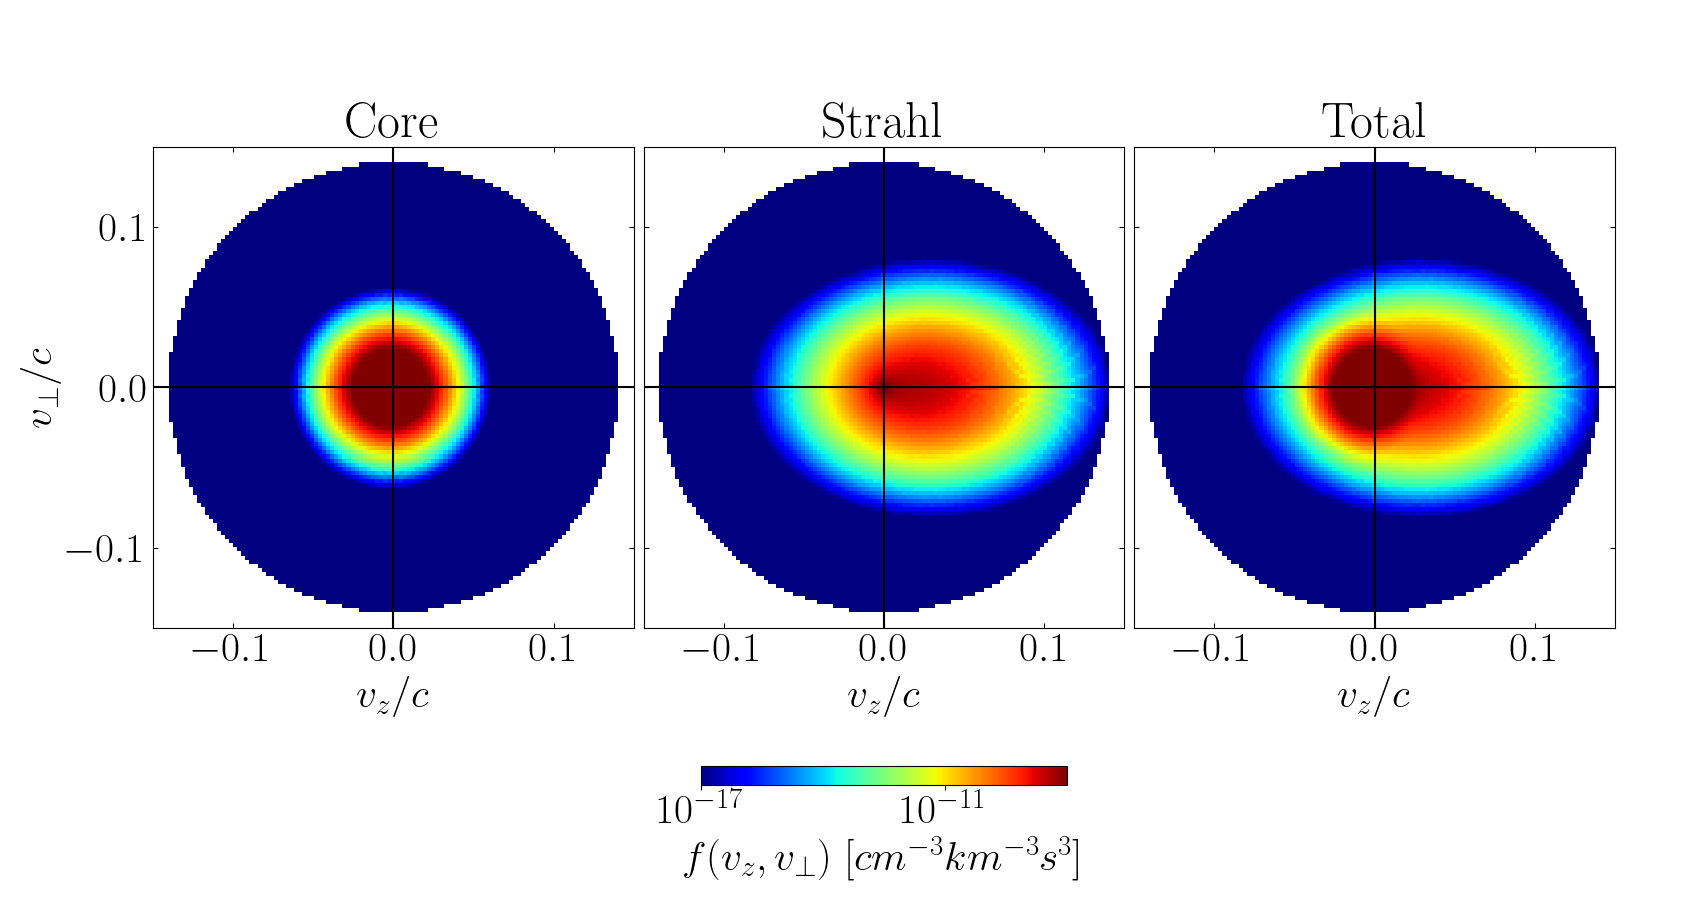
\includegraphics[width=\textwidth]{original_0.3_AU.png}
    \caption{Model of initial electron populations at 0.3 AU used in the
        simulations in \cite{Micera2020}. The core and
    strahl bulk velocity ensures zero net current.}
    \label{fig:03_AU_particles}
\end{figure}

In the velocity distribution of solar wind electrons, observations have shown
that there are usually three populations, a cold core, a hot halo, and a magnetic field aligned strahl, which evolve with heliospheric distance
\citep{Montgomery1968,Feldman1975,Pilipp1987}. Observations near the Sun (0.3 AU) from the Parker Solar Probe (PSP) have reported that the halo almost disappears, while the strahl is narrower than further out from the Sun \citep{Halekas2020}. \cref{fig:03_AU_particles} shows an example of the velocity
distribution function (VDF) of electrons at 0.3 AU, where both core and
strahl populations are modelled with a bi-Maxwellian distribution. Far from the
Sun, statistical studies at 1 AU from \cite{Maksimovic2005} and \cite{Wilson2019} have modelled core electrons with a bi-Maxwellian distribution, while the halo and the strahl are better fitted with a bi-Kappa distribution (see \cref{fig:solar_wind_electrons}).
\begin{figure}
    \centering
    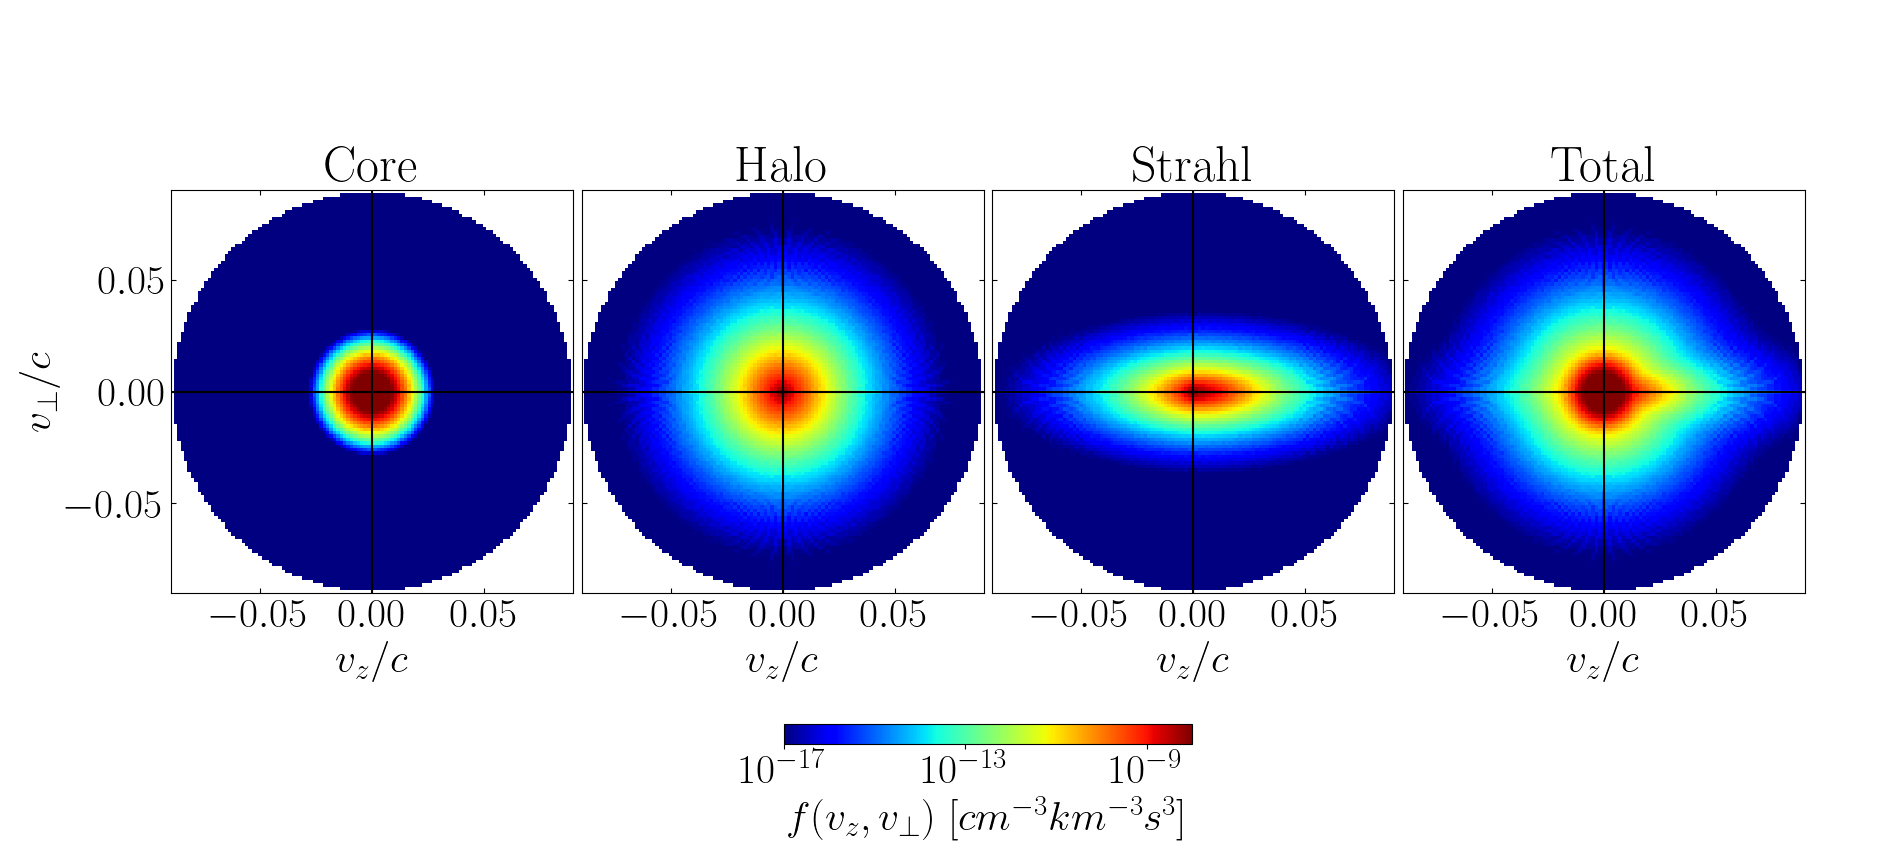
\includegraphics[width=\textwidth]{original_1_AU.png }
    \caption{Components of solar wind electrons
observed by the Wind satellite at 1 AU as fitted by \cite{Wilson2019}.}
    \label{fig:solar_wind_electrons}
\end{figure}

As these electrons stream radially out, if their propagation were adiabatic,
meaning the magnetic moment $\mu\sim v_\perp^2/B_r$ were conserved, then the
perpendicular velocity would have to decrease. This means far from the Sun, the
strahl should be increasingly narrow. However, in-situ data have shown an
opposite trend in the radial evolution of solar wind electrons.
\cite{Stverak2009} observed from 0.3 to 1 AU that the strahl density decreased
as the halo density increased by the same amount relative to the core (see
\cref{fig:density_radial_evolution}). This suggests that the origin of the halo
is due to the scattering of the strahl. Additionally, \cite{Anderson2012} and
\cite{Graham2017} reported that the strahl's pitch angle width distribution
varied greatly from 5 to 90$^\circ$ at 1 AU and increased radially beyond 1 AU.
Thus, it would be harder to identify a field aligned strahl population further
out from the Sun.

\begin{figure}
    \centering
    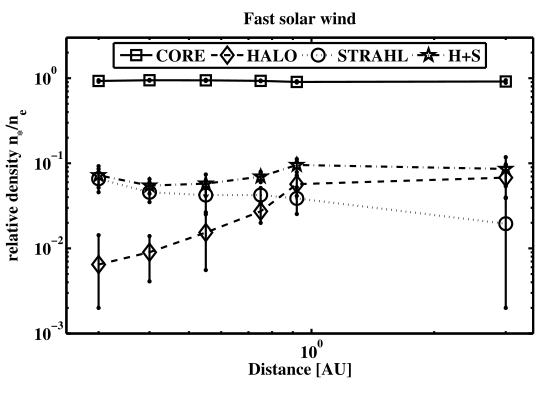
\includegraphics[width=0.48\textwidth]{density_evolution_fast.png}
    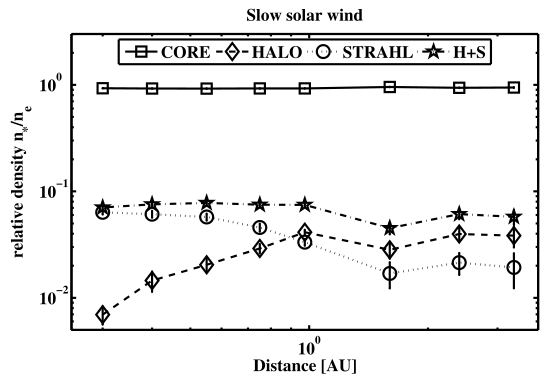
\includegraphics[width=0.497\textwidth]{density_evolution_slow.png}
    \caption{Radial evolution of electrons in the fast and slow
    solar wind from 0.3 to 6 AU \citep{Stverak2009}.}
\label{fig:density_radial_evolution}
\end{figure}

Therefore, there must be a mechanism that scatters strahl
electrons into the halo distribution. Wave-particle interaction is one such
process that allows the energization and scattering of resonant electrons.
Specifically, whistler-mode waves, a right-hand polarized electromagnetic wave,
have long been proposed as a candidate to explain these solar wind observations.
Through theoretical and simulation studies, they have been demonstrated to
scatter electrons in the Earth's radiation belts \citep[][and references
therein]{Karimabadi1990,Albert1993,Tao&Bortnik2010,Hsieh2017}. However,
these studies typically focused on small whistler amplitudes with $\delta
B/B_0\sim\mathcal{O}(10^{-4})$. \cite{Breneman2010} and \cite{Cattell2020} used
electric field waveform captures from the STEREO satellites at 1 AU and
demonstrated that large amplitude, narrowband, obliquely propagating whistlers
were frequently present in the solar wind. They were observed in the range of
$5$--$40$\,\si{mV/m}, which corresponds to $\delta B/B_0\sim\mathcal{O}(0.1)$.
These large amplitude whistlers recently became an interest because of
new data from the PSP at 0.3 AU. \cite{Agapitov2020} and \cite{Cattell2021} 
observed large amplitude waves of this order near the Sun. Additionally, their
polarization indicated that the propagation varied from quasi-parallel to
oblique angles. \cite{Micera2020} simulated whistlers from heat-flux
instabilities near the Sun using electron distributions modeled after PSP
data and showed the halo formation from strahl electrons. \cite{RobergClark2019} reported the formation of ``horns'' in
velocity space due to the scattering of resonant strahl electrons with oblique
whistlers in solar flares (see \cref{fig:vdf_horns}). Thus, we are interested in
studying the scattering and energization of solar wind electrons due to these
large amplitude waves and comparing our results with observations and these recent simulations.

\begin{figure}
    \centering
    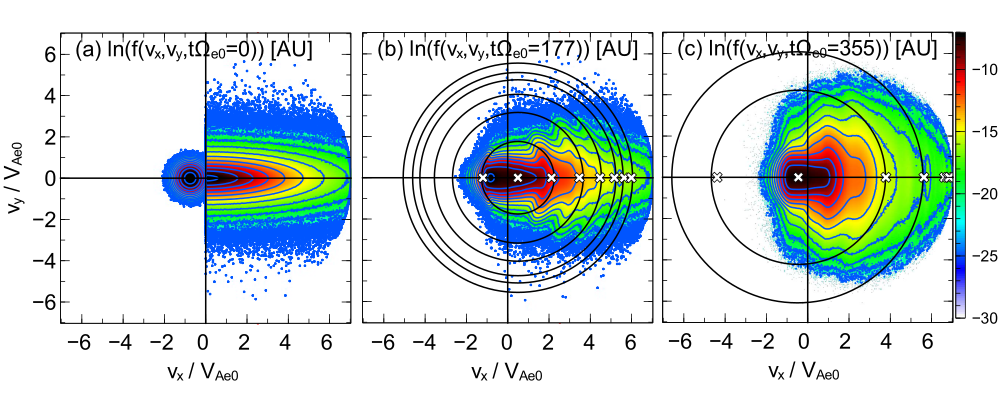
\includegraphics[width=\textwidth]{vdf_horns.png }
    \caption{Formation of horns in velocity space of an
        original distribution (a) of core and strahl
        electrons \citep{RobergClark2019}. The horizontal and vertical axes are
    the parallel and perpendicular velocity normalized by the electron Alfvén
    speed. Panel (b) shows the resulting interaction with a right-ward wave.
The white crosses are the $n=-5,-4,...,1$ resonances. Panel (c) shows that with
a left-ward wave (with $n=-1,0,...,5$ resonances).}
    \label{fig:vdf_horns}
\end{figure}


%\begin{figure}
%    \centering
%    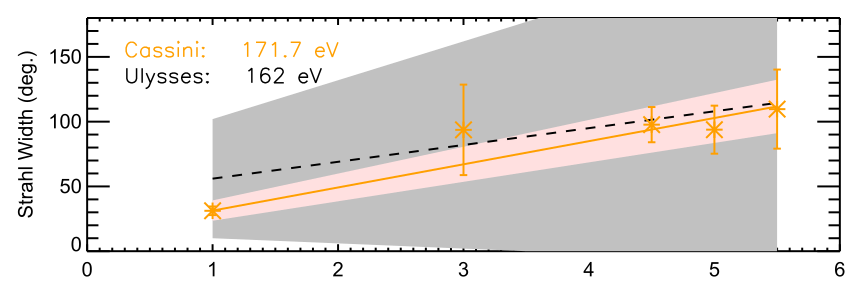
\includegraphics[width=\textwidth]{strahl_width.png }
%    \caption{Radial evolution of the strahl's pitch angle width beyond 1AU \citep{Graham2017}.}
%    \label{fig:strahl_width}
%\end{figure}

\cite{Kersten2014} developed a test particle
simulation to study whistler-electron interactions in the radiation belts
and later adapted it to simulate whistlers at stream interaction regions in the
solar wind based on observations in \cite{Breneman2010}. Modelled after the
simulation in \cite{Roth1999}, the code used a fourth order Runge-Kutta (RK)
integration algorithm to solve the Lorentz equation numerically. This is a
general approach to numerical problems as the RK family of integrators is known
to produce highly precise solutions. The results are therefore reliable as long as one is interested in single-particle behaviors. However, this approach fails to maintain the consistency among a spectrum of initial conditions as the solutions might be more unstable for certain regions in phase space. For the high amplitude waves of interest, chaotic behavior is usually present. Thus, this program is insufficient to investigate the behavior of an electron distribution as it provides no physical measure to judge the reliability among the results.

Particle-In-Cell (PIC) simulations, as used by \cite{Micera2020} and
\cite{RobergClark2019}, are a standard in plasma research in studying
self-consistently evolving systems. Instead of a high order RK algorithm, they
usually use a time-centered, second-order explicit integrator called the Boris
pusher \citep{Birdsall&Langdon1985}. Although not a symplectic algorithm,
it is the \textit{de facto} method for advancing a charged particle in an
electromagnetic field because the Boris pusher conserves local phase space
volume \citep{Qin2013}. This means the energy error is globally bounded for an
arbitrarily large number of time steps. Thus, this numerical method is capable
of resolving multi-scale dynamical problems over a long simulation period.
However, PIC simulations are computationally expensive, as they solve Maxwell
equations along with advancing particles and usually handle millions to
trillions of particles. For our purpose, large scale PIC simulations are not
necessary, because test particle simulations allow us to examine the interaction
for different wave properties and over all particle angles and energies.


In this thesis, a vectorized test particle simulation capable of
investigating the behavior of a distribution of hundreds of thousands of
electrons is utilized. The code is modelled after the Vector Particle-In-Cell 
(VPIC) code using only the particle advancing component \citep{Bowers2008}. In
\cref{sec:theory}, a derivation of the whistler wave fields from a cold, 
collisionless plasma dispersion relation is given. Also, the Hamiltonian
analysis of the resonance surface using Hamilton-Jacobi and perturbation theory
is discussed. In \cref{sec:simulation}, detail of the calculations in the
simulation are laid out, together with the estimation of the Lyapunov exponents 
to measure the efficiency of the integration algorithm.
\cref{sec:diagnostics} presents the diagnostics of the simulation including the 
Lyapunov exponents, the adiabatic invariants, and whistler parameters. 
\cref{sec:analysis} reports simulation results of the electron distribution 
interactions with single uniform whistlers and a narrowband packet of whistlers 
at 0.3 AU and 1 AU and their analysis as according to quasi-linear
resonant theory. Conclusions and suggestions for future works are in
\cref{sec:conclusion,sec:future_works}.
